\chapter{Belle II Upgrade} \label{ch:upgrade}

This second chapter wants to address the motivation for the upgrade of Belle II. We will give an overview of the primary background sources in the experiment to understand how to mitigate them in order to achieve a better performance of the whole detector, when ramping up the luminosity. We will also introduce some of the proposals made for the improvement of the vertex detector.


%---------------------------------------------
%			2.1
%---------------------------------------------

\section{Purposes of the upgrade}

The physics program of the experiment requires SuperKEKB to work under challenging conditions and machine backgrounds play an important role in the safety, efficiency, and performance of data taking. 
Current studies \cite{Natochii:2022vcs} predict that the accelerator may reach higher luminosity targets with the existing accelerator complex, but to achieve the established final value of \SI{6e35}{cm^{-2} s^{-1}}, an enhancement of the interaction region is being considered.\\
Several improvements and modifications have been planned during two long shutdowns in order to reach the integrated luminosity target of \SI{50}{ab^{-1}}: LS1 in 2022 to install a complete VXD, and LS2 in 2028 or later for the upgrade of the interaction region and the accelerator components. LS2 offers the opportunity for a significant detector upgrade, improving robustness against backgrounds and physics performance.

Belle II detector is expected to operate efficiently under the levels of background extrapolated to luminosity target, but safety margins are not large. Moreover, in case of a redesign of the interaction region large uncertainties in the background extrapolations are unavoidable. \\

Therefore the global upgrade program \cite{Forti:2022mti} is justified by many considerations, among them:

\begin{itemize}
\item improve detector's resistance to higher levels of background;
\item make subdetectors more robust against radiation damage;
\item push forward safety margins for running at higher luminosity;
\item develop the technology to cope with different future paths;
\item improve overall physics performance.
\end{itemize}


%---------------------------------------------
%			2.2
%---------------------------------------------
\section{Background sources and limitations in \\Belle II}

SuperKEKB is already the world's highest-luminosity collider and it aims to reach a new peak in the near future and to increase the collected statistics, to become more sensitive to rare processes and precise measurements of Belle II physics program. 
But to be able to do this without loosing the good functionality of the entire detector, it is necessary to understand how to reduce the beam background where possible and how to cope with the consequent challenges.

Several simulations and measurements of beam background \cite{Natochii:2023thp} are being done in order to guess possible future machine scenarios, under new luminosity conditions.
This is necessary to study the vulnerability of the subdetectors (and more generally of the machine) and thus, to design the countermeasures to adopt against the deterioration of performance and materials.


\subsection{Main background sources}

In the following some of the primary \textit{single-beam} and \textit{luminosity-dependent} background sources are discussed \cite{physics_book, Natochii:2022vcs}.


\begin{description}
\item[Touschek effect]: 
	It is an intra-bunches scattering process, where the Coulomb scattering of two particles in the same beam bunch causes a variation of their energies, increasing the value of one of them and lowering that of the other from the nominal value. This interaction among the bunch particles is the first beam background source at SuperKEKB.
\item[Beam-gas scattering]: 
	this represents the collision of beam particles with residual gas molecules in the beam pipe. It is the second beam background source and it can occur via two processes: \emph{Coulomb interaction}, which changes the direction of the beam particles and \emph{bremsstrahlung scattering}, which decreases their energy. 
\end{description}
	
In these two processes, the scattered particles fall out the stable orbit and hit the beam pipe while they move around the ring. This mechanism causes electromagnetic showers that can reach the detector if their origin (loss position) is near the interaction region. Collimators are in place to reduce these backgrounds by absorbing the off-orbit particles. These backgrounds are present even if the beams are not colliding and are therefore called \textit{single-beam} backgrounds.


\begin{description}
\item[Radiative Bhabha scattering]:
	It is the electron-positron scattering $e^{+}e^{-} \rightarrow e^{+}e^{-} \gamma$, an undesirable collision process at the IP which has very high cross section but only little interest for the physics studied in the experiment.
	The emitted photon can interact with the magnets near the detector producing a large amount of neutrons via the photo-nuclear resonance mechanism (such neutrons are the main background source for the outermost Belle II detector).\\
	
\item[Two-photon process]:
	it consists in the process $e^{+}e^{-} \rightarrow e^{+}e^{-}e^{+}e^{-} $. The produced electron-positron pairs can spiral around the solenoid field lines and leave multiple hits in the inner layers of the detector.\\
	
These backgrounds are called \textit{Luminosity backgrounds} because their strength is proportional to the luminosity. They can be reduced with a careful design of the interaction region including neutron shielding.

\item[Synchrotron Radiation (SR)]:
	X-rays emitted from the beam when electrons and positrons pass through the strong magnetic field near the IP. The HER beam is the main source of this type of background, because SR power is proportional to the square of beam energy and magnetic field.
SR can potentially damage the inner layers of the vertex detector due to an higher radiation dose in that region. Absorbing structures have been implemented inside the beam pipe to protect the detector from SR.
\end{description}

The rate of these processes is relatively high for small beams and high currents, leading to a beam lifetime in the order of only few minutes. This requires a continuous injection mechanism, in which particles are added to individual bunches to keep the charge constant. While this is essential for high luminosity operation, it is also the source of an additional background, since the perturbed bunches are noisy for a number of turns. The injection background is particularly hard to model and estimate.

\subsection{Current background status and future predictions}\label{sec:bkg_predictions}

Several monitoring devices are located all along the accelerator to measure radiation doses on the detector and delicate regions of the ring, in order to intervene as soon as possible in case too high levels are reached.

Dedicated beam background studies have been performed and for example, \autoref{fig:bkg_plot} shows the rates measured in June 2021 \cite{Natochii:2023thp} with a betatron function at the IP of $\beta_{y}^{*}$ = \SI{1}{mm} and a collision luminosity of \textit{L} = \SI{2.6e34}{cm^{-2} s^{-1}}. Current background rates in Belle II are acceptable and in most cases, well below the limits listed in~\autoref{tab:bkg_table} \cite{Natochii:2022vcs}.\\

\begin{figure}[h!]
\centering
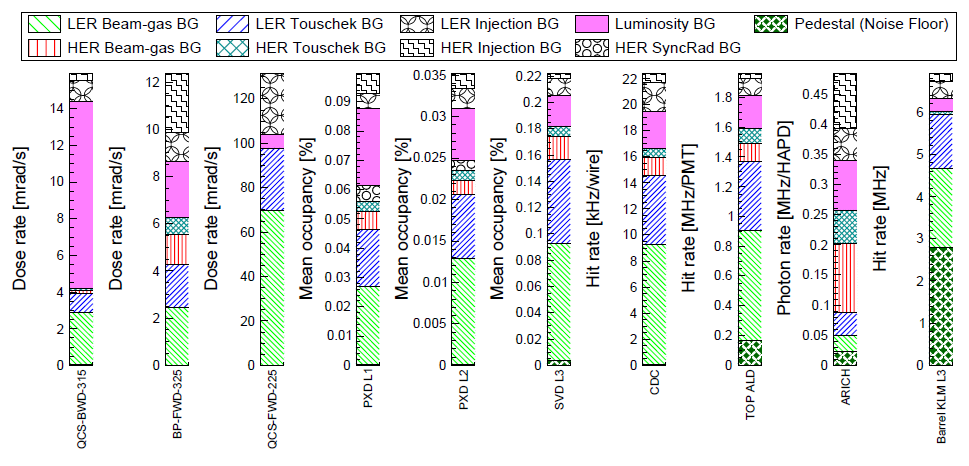
\includegraphics[scale=.7]{bkg_plot}
\caption{Measured Belle II background in June 2021. Each column shows different background sources for Belle II sub-detectors, for superconducting quadrupole magnet (backward and forward) and for the beam pipe.}
\label{fig:bkg_plot}
\end{figure}


\begin{table}[htb]
\centering
    \begin{tabular}{lccc}
    \hline\hline
    Detector & \multicolumn{2}{c}{BG rate limit} & Measured BG\\
    \hline
    Diamonds & \multicolumn{2}{c}{\SIrange{1}{2}{rad/s}} & $<\SI{132}{mrad/s}$\\
    PXD & \multicolumn{2}{c}{\SI{3}{\%}} & \SI{0.1}{\%}\\
    SVD L3, L4, L5, L6 & \multicolumn{2}{c}{\SI{4.7}{\%}, \SI{2.4}{\%}, \SI{1.8}{\%}, \SI{1.2}{\%}} & $<\SI{0.22}{\%}$\\
    CDC & \multicolumn{2}{c}{\SI{200}{kHz/wire}} & \SI{22.3}{kHz/wire}\\
    ARICH & \multicolumn{2}{c}{\SI{10}{MHz/HAPD}} & \SI{0.5}{MHz/HAPD}\\
    Barrel KLM L3 & \multicolumn{2}{c}{\SI{50}{MHz}} & \SI{4}{MHz}\\
    & \multicolumn{2}{c}{non-luminosity BG} &\\\cline{2-3}
    & Before LS1 & After LS1 &\\\cline{2-3}
    TOP ALD & \SI{3}{MHz/PMT} & \SI{5}{MHz/PMT} & \SI{1.8}{MHz/PMT}\\
    & \multicolumn{2}{c}{+ luminosity BG} &\\
    \hline\hline
    \end{tabular}
    \caption{Background rate limits for Belle II detector sub-systems. The third column shows the total measured background rate in June 2021}
    \label{tab:bkg_table}
\end{table}


Event though the current level is of no concern in terms of occupancy for the innermost layers of the vertex detector, a larger amount of localized SR, for example, could cause inhomogeneities in PXD modules, which would be very difficult to compensate by adjusting the operation voltages of the affected ones.\\

Until now it can be said that SuperKEKB and Belle II are operating stably. Beam-induced background rates are well below the limits of the detector and do not prevent from increasing further the current and hence the luminosity, as demonstrated by the predictions for the background rates \textit{before LS2} with a known machine configuration. 
For what concern the predictions at \textit{$L_{inst}$} = \SI{3e35}{cm^{-2}s^{-1}} instead, called \textit{after LS2} operation, there are several uncertainties tied to the machine configuration. In fact at the moment, the working machine lattice to reach the target luminosity is not known and in addition, the final design of the IR and beam pipes is not concluded yet.

Therefore an alternative solution is employed to roughly estimate the background rates. The background predicted Before LS2 phase is considered as a starting point and then different scaling factors are applied for single-beam background component, considering three different possible scenarios:

\begin{itemize}
\item \textbf{x2} - optimistic scenario-1 (\textbf{v1})
\item \textbf{x5} - nominal scenario-2 (\textbf{v2})
\item \textbf{x10} - conservative scenario-3 (\textbf{v3}), an arbitrary factor assuming that all single-beam backgrounds will be increased by a order of magnitude After LS2.
\end{itemize}

The luminosity background sources are instead scaled with luminosity ratio.
These are then used to simulate the behaviour of the whole detector in future perspectives, as we will see in the following.


%---------------------------------------------
%			2.3
%---------------------------------------------
\section{Summary of possible VXD upgrade} \label{sec:VTX_requirements}

The Vertex Detector is particularly sensitive to machine background because it is the closest to the beam pipe and therefore subject to high doses of radiation.
As we have already seen, current studies are trying to extrapolate how it could be affected by reaching the future luminosity target, but there are a lot of uncertainties due to models and still not well defined design of the interaction region. Moreover, a completely new detector might be required in the event of a considerable redesign of the IR, and the physics performance could be also improved, taking advantage of the more recent technology developments.\\
In particular, all different upgrade ideas of the entire Belle II detector intend to ensure its proper functioning at the higher levels of luminosity, considering also further improvements of the lattice machine and the colliding beams. The current detector configuration is not expected to maintain its performance when facing higher beam background levels or higher rates.\\

Concerning the Vertex Detector, all proposed improvements aim to:

\begin{itemize}
\item reduce occupancy level by employing fully pixelated and fast detector (CMOS technology has been chosen);
\item increase robustness against tracking efficiency and resolution losses from beam background;
\item improve radiation hardness to reduce detector ageing effects and performance degradation;
\item reduce the inserted material budget between subdetectors in order to achieve good resolution by lessening the multiple scattering, especially important at lower momenta.
\end{itemize}


In the following we will present in a few words the four main proposals for future upgrade: Depleted Field Effect Transistor (DEPFET) pixel, thin strip sensor, CMOS Monolithic Active Pixel Sensor and SOI technology.
The first two are more conservative and try to exploit as much as possible of the existing detector, making some appropriate adjustments to the sensor type, readout or mechanical structure. The last ones instead, plan to build an entirely new detector.\\

The reference background levels determining radiation robustness requirements of the innermost layers are the following:

\begin{itemize}
\item Hit rate capability: \SI{120}{MHz/cm^{2}};
\item Total Ionizing Dose: \SI{10}{Mrad};
\item NIEL fluence: \SI{5e13}{n_{eq}/cm^{2}}.
\end{itemize}

At this time, the main effort is focused in the development of the CMOS MAPS system, with the SOI as a possible backup option, although still requiring significant R\&D. The DEPFET and thin strip sensors are substantially abandoned, but we present them here to provide the full picture.


\subsection{Depleted Field Effect Transistor (DEPFET)}

This first proposal intend to minimize risks and costs of the project, preserving the general layout of the PXD system. The upgrade consists to improve the sensor to provide higher safety factor for the allowed occupancy and to prevent some issues that currently weaken the good functionality of the detector.

Some of the main improvements are listed below:

\begin{itemize}
\item improve signal transmission on the pixel matrix and the signal processing in the readout, in order to reduce the readout time per row from the current \SI{100}{ns} to \SI{50}{ns}. In this way the frame time and the background occupancy might be reduce by a factor 2, while leaving unchanged the optimized size and the number of PXD pixels;
\item increase the robustness against beam losses which could make the gate lines inefficient or even inoperative, on almost all PXD modules. This reaction seems to be due to a high photocurrent on the chip because of the high instantaneous dose. It could be mitigated by adding protection circuits on-chip;
\item Total Ionizing Dose (TID) effect on the chip provokes an unexpected avalanche current that does not compromise the sensor performance, but requires more power supply to provide enough current. This issue might be solved by bringing some changes in the DEPFET pixel layout.
\end{itemize}

The DEPFET improvement R\&D is currently inactive because of lack of person power and dedicated funding.

\subsection{Thin and Fine-Pitch SVD}

The Thin and Fine-Pitch SVD (\textbf{TFP-SVD}) is a new detector concept that aims to improve not only SVD, but potentially also the inner part of the CDC, whose functionality could be threatened by future beam background conditions.
This proposal uses Double-sided Silicon Strip Detectors (DSSDs) for the inner and middle detector volume, since a single sensor can cover large dimensions. In the current detector the DSSD technology is already used in the SVD. \\

The major improvement would be the reduction of the material budget.
Currently SVD has about 0.7\% $X_{0}$ material budget per layer. TFP-SVD instead, decreasing the sensor thickness to \SI{140}{\micro m}, intends to reduce it to 0.41\% $X_{0}$. 
Moreover, a smaller sensor thickness is expected to reduce the voltage needed to reach the full depletion, even after radiation damage. 
The front-end developed for TFP-SVD, the SNAP128 chip, offers also a reduction of the amount of cables.

%has 128 input channels with a \SI{127}{MHz} clock binary hit information sampled. It also offers a reduction of the amount of cables.

Some concerns about TFP-SVD are the feasibility and efficiency of the final sensor production and the small signal charge due to the short path length of the particles through the sensor.

A first prototype has been produced by Micron-Semiconductor Ltd (UK), with a size of \numproduct{52.6 x 59.0}~\unit{mm^{2}}. The characterization studies are in agreement with the expectation and also a lower full depletion voltage is confirmed.
The development of the TFP-SVD option has been abandoned because of the small signal to noise ratio (10 or less) and difficulties in the chip design optimization.


\subsection{CMOS Monolithic Active Pixels Sensor}

The VTX proposal, that we will analyze in more details in the next chapter, aims to replace the entire current VXD detector using Monolithic Active Pixel Sensors (MAPS) based on CMOS (Complementary Metal-Oxide Semiconductor) technology. \\
In CMOS MAPS the basic commercial CMOS technology is minimally modified to allow the collection of the charge released by a charged particle traversing the epitaxial layer where the readout electronics is fabricated. There are many technological variant sharing this same concept.

\begin{comment}
The program hopes to solve some of the issues discussed in the previous chapters, with a new system of two inner layers and three outermost, for a total of 5 stages equipped with a single sensro type, called \textbf{VTX} (layout in~\autoref{fig:VTX_layout}). Also the mechanical structure has been redesigned but it is expected that the all system could work at room temperature, so as consequence an important reduction of services is also contemplated.\\
\end{comment}

The Belle II chip is called OBELIX (Optimized BELle II pIXel sensor), based on the pixel matrix of the TJ-Monopix2 chip, whose characterization is the main topic of this work (Chapter 5) and which is developed with the technology of the TowerJazz company with a minimum feature size of \SI{180}{nm}. 
The size of the sensor is expected to be \numproduct{3 x 1.9}~\unit{cm^{2}} with a pixel pitch between \SI{30}{\micro m} and \SI{40}{\micro m}, achieving a spatial resolution below \SI{15}{\micro m}, required by the VTX upgrade program. The timestamp clock signal have to reach down to \SI{25}{ns}, in order to deal with the target hit rate of \SI{120}{MHz/ cm^{2}}. All these characteristics allow to obtain a sensor with high granularity in time and space.\\

The VTX detector consists in 5 concentric layers of monolithic sensors with a barrel geometry. The global target thickness for the air-cooled two inner layers and for the water-cooled three outer layers, is expected to be of about 2\%$X_{0}$.

\begin{figure}[h!]
\centering
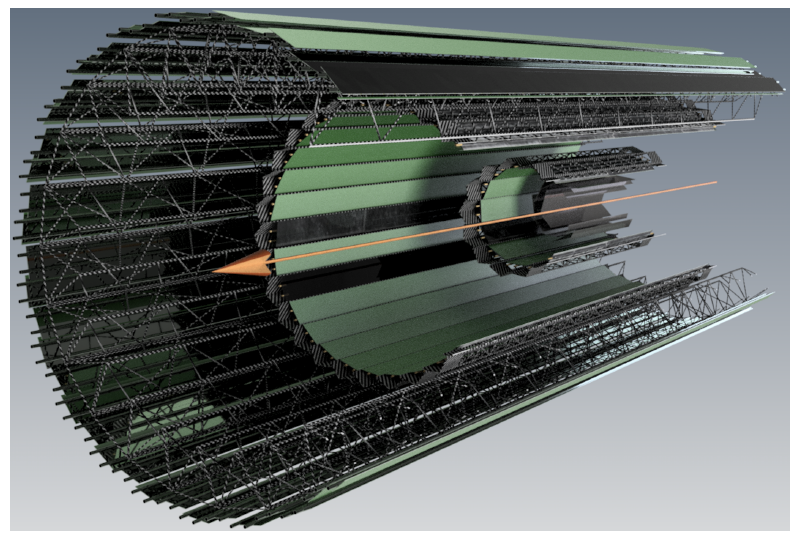
\includegraphics[scale=.6]{VTX_layout}
\caption{Overall VTX layout.}
\label{fig:VTX_layout}
\end{figure}

The VTX solution intends to reduce the current PXD integration time by at least two orders of magnitude introducing also other improvements:

\begin{itemize}
\item lower detector occupancy which allows to cope with higher background and to mitigate data-transmission bottlenecks.
\item Better tracking efficiency and improved momentum resolution and impact parameter resolution at low transverse momentum.
\item Smaller data cables cross sections and less complex cooling system which might lighten the needed services.
\item Simplified control and power systems due to the use of a single sensor chip for all layers.
\end{itemize}

At the current state of art intense R\&D is being carried out, taking advantage from the experience of other experiments like ALICE, with the same type of sensor \cite{Fantoni:2020iyr}.\\


\subsection{Silicon On Insulator (SOI)}

An alternative proposal employs a new pixel design, called Dual Timer Pixel (DuTiP) \cite{Ishikawa:2020gpo}, based on SOI technology (see~\autoref{sec:SOI_tech}). In Silicon-On-Insulator (SOI) technology, electronics is fabricated in a silicon layer separated by a \ch{SiO_2} isolation layer from the main detector substrate.
This new sensor concept has been developed to fulfill the requirements of a new vertex detector with faster readout, lower occupancy, smaller data size and smaller data transfer. In particular, it aims to store at least two hits during the Belle II trigger latency (\SI{5}{\micro s}), to avoid loss information in higher background environment. 

The size of the new designed pixel is \SI{45}{\micro m} and the sensor layer thickness is \SI{50}{\micro m}, which gives an intrinsic resolution better than \SI{15}{\micro m}. The analog part is quite standard for a binary detector and consists of a sequence of preamplifier, shaper and comparator. ALPIDE \cite{AGLIERIRINELLA2017583} was choosen as analog circuit with some modifications to adapt it to SOI technology. 
The quite complex digital circuit has to be assembled on each pixel, and Lapis semiconductor \SI{2.0}{\micro m} FD-SOI CMOS technology has been chosen, based on the experience gained in the successful development of other detectors like the pixel detector for the future ILC (SOFIST) \cite{Murayama:2020ujz}.

DuTiP pixel detector is designed to cover the current VXD acceptance with 7 layers. For the inner layer of the detector might be possible the cooling with airflow at room temperature; for the outer layers instead, a combination of air and water flows. The DuTiP R\&D are ongoing and the chip prototypes seems to work fine, in agreement with the expectations, although there are concerns about the radiation hardness of the technology. \\

After this brief review of the main upgrade proposals, we can then elaborate on the VTX program in \autoref{ch:VTX}.

























\begin{comment}

on \textit{z} direction averaging over incident polar angle

\begin{description}
\item \textbf{Concept}
\end{description}

SOI technology has been chosen as baseline for the new pixel design thanks to its monolithic structure, thinness, low power consumption and low parasitic capacitance. In addition it is resistant aginst neutron and single event upset (SEU\footnote{A Single Event Upset (SEU or SEE, Single Event Error) occurs when a ionizing particle deposits charge close to a storage node (e.g. RAM cell, register) causing a bit value to flip leading to corrupt information. This effect could be mitigated by using, for example, redundant memory. It is not a permanent damage. \label{foo:SEU}}), even though an important issue is TID effect on which efficient solutions have been studied.

When a processed hit signal arrive to the digital part it is stored and one of the timers start to counting down from a starting time set to trigger latency plus one clock, waiting for trigger signal. If the trigger signal is received when the time is 1 (it could be also 2 or 0), the signal is readout as \emph{Current} (\emph{Next} or \emph{Previous} respectively) timing (\emph{PCN timings}). If the trigger is not received at the PCN timings in the pixel, the timer is reset. 

\begin{figure}[h!]
\centering
\subfigure[Analog, Digital and Scan blocks for DuTiP detector.]{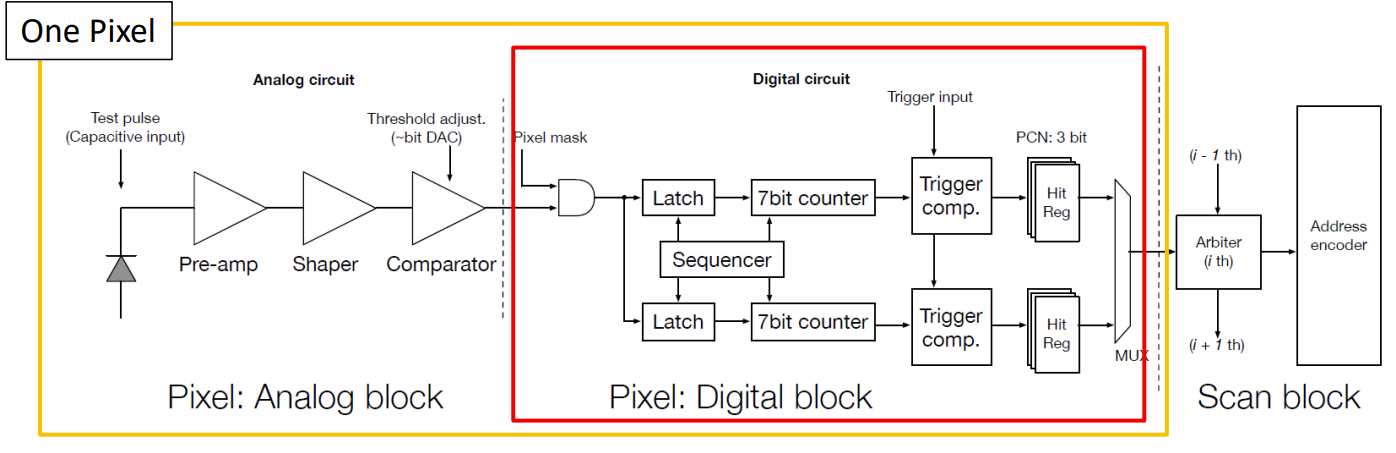
\includegraphics[scale=0.3]{SOI1}}\quad
\subfigure[Operational sketch.]{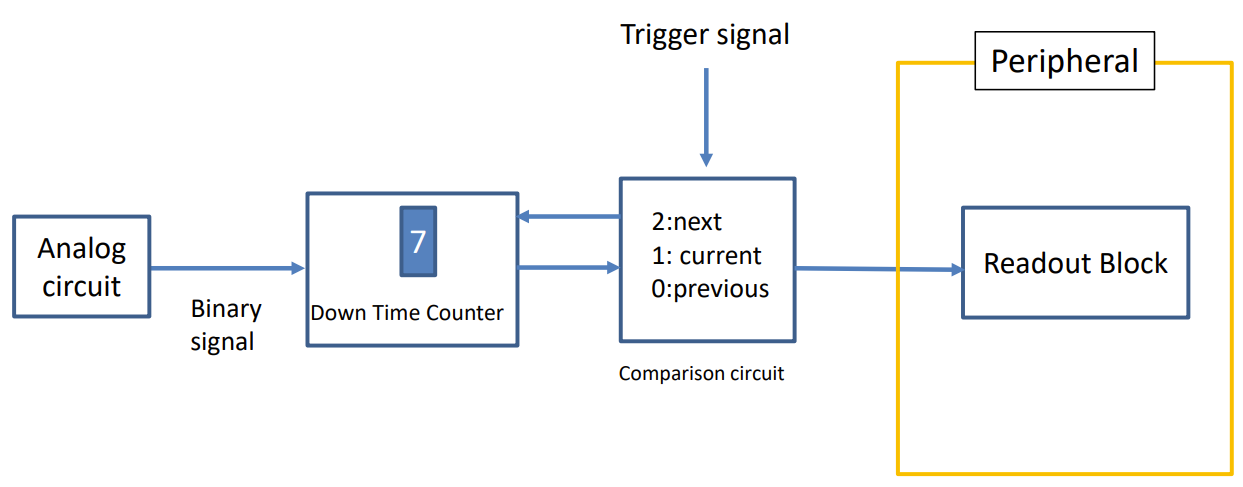
\includegraphics[scale=0.4]{SOI2}}\\
\caption{Schematic of DuTiP circuits.}
\label{SOI}
\end{figure}


\begin{description}
\item \textbf{Sensor design and and features}
\end{description}

DuTiP pixel detector is designed to cover the current VXD acceptance with 7 layers: 1-3 with S (smaller size chip) type sensors, 4-7 with L(larger size) type (\autoref{fig:SL_SOI}).

\begin{figure}[h!]
\centering
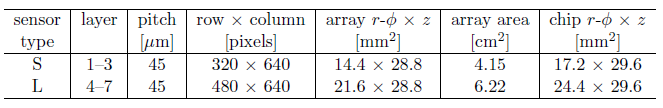
\includegraphics[scale=1]{SL_SOI}
\caption{The size of Small (S) and Large (L) DuTiP chips.}
\label{fig:SL_SOI}
\end{figure}

Stitching technique allows to produce longer chips in the \textit{z} direction, but the structure of the ladders has not be decided yet. Anyway the target is to minimize the dead region between chips in the ladder. 

For layer 1, which is expected to work in more severe condition of background, the pixel occupancy has been estimated with the trigger latency of 8.0 $\mu$s and for both L and S type it is small enough, O($10^{14}$) or less, thus stable tracking and vertexing are contemplated. Moreover without using two timers for layer 1, the signal loss probability with the trigger latency of 4.5 (8.0) $\mu$s is about 0.2 (0.4)\% and so not negligible. In fact if the background rate is higher and the latency is longer, the signal loss probability increases.\\ 

The first prototype of this new chip has been delivered in June 2021, with all in-pixel functionalitites except for the scan block and the fast readout system. The chip is a matrix of \numproduct{64 x 64} pixels and size of \numproduct{6 x 6} $mm^{2}$. Its characterization is ongoing and it seems to work fine, aslo with radioactive sources and red laser tests. \\
The second prototype DuTiP2 had been delivered in 2022, with \numproduct{32 x 320} pixels and size of \numproduct{17.2 x 6} $mm^{2}$. It has all functionalities except for fast hit data collection to periphery. The phase of testing is ongoing.
A third prototype has been submitted in 2023 and will be delivered in 2024 (all prototypes shown in~\autoref{fig:dutip_matrix}).

\begin{figure}[h!]
\centering
\subfigure[DuTip1 prototype on the left and DuTiP2 on the right.]{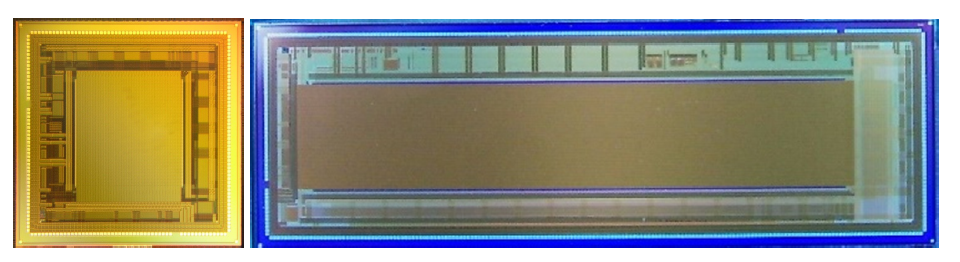
\includegraphics[scale=0.7]{DuTiP12}}\quad
\subfigure[DuTip3 third protoype.]{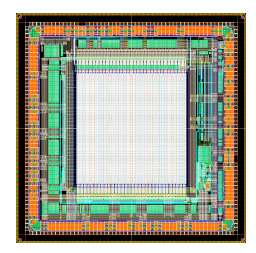
\includegraphics[scale=0.8]{DuTiP3}}\\
\caption{DuTiP prototypes.}
\label{fig:dutip_matrix}
\end{figure}
\end{comment}
